\documentclass[tikz,border=14pt]{standalone}
\usetikzlibrary{arrows.meta,positioning}
\begin{document}
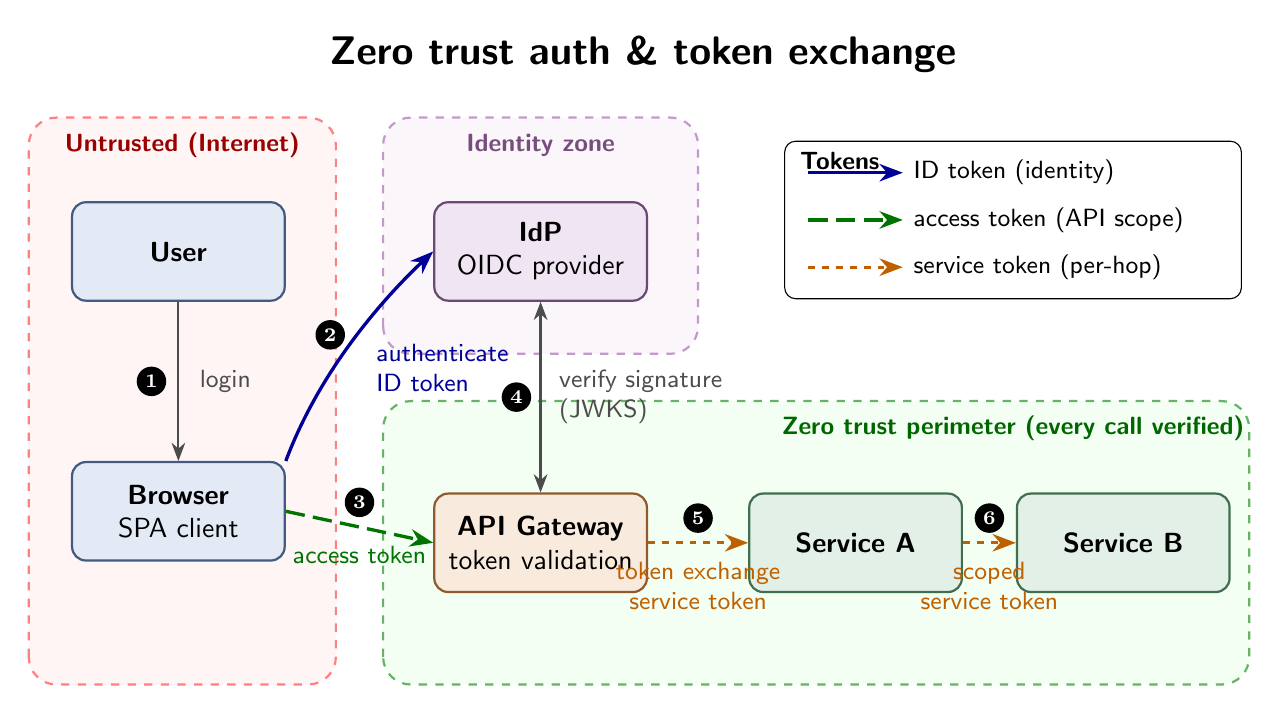
\begin{tikzpicture}[
  >=Stealth,
  font=\sffamily,
  box/.style={draw=#1!65!black,fill=#1!18,rounded corners=5pt,
    minimum width=2.7cm,minimum height=1.25cm,align=center,thick},
  idtok/.style={->,very thick,blue!60!black},
  actok/.style={->,very thick,green!45!black,dash pattern=on 7pt off 3pt},
  svtok/.style={->,very thick,orange!75!black,dash pattern=on 2.5pt off 2.5pt},
  plain/.style={->,thick,gray!60!black},
  lab/.style={font=\small\sffamily},
  stepnum/.style={circle,fill=black,text=white,inner sep=1.5pt,font=\scriptsize\bfseries}]

  \definecolor{userc}{RGB}{100,140,200}
  \definecolor{idpc}{RGB}{170,110,180}
  \definecolor{gwc}{RGB}{220,140,70}
  \definecolor{svc}{RGB}{100,170,120}

  % ---- trust boundaries ----
  \fill[red!4,rounded corners=10pt] (-1.9,-1.6) rectangle (2.0,5.6);
  \draw[red!50,thick,dashed,rounded corners=10pt] (-1.9,-1.6) rectangle (2.0,5.6);
  \node[font=\small\sffamily\bfseries,text=red!60!black] at (0.05,5.25) {Untrusted (Internet)};

  \fill[idpc!6,rounded corners=10pt] (2.6,2.6) rectangle (6.6,5.6);
  \draw[idpc!70,thick,dashed,rounded corners=10pt] (2.6,2.6) rectangle (6.6,5.6);
  \node[font=\small\sffamily\bfseries,text=idpc!70!black] at (4.6,5.25) {Identity zone};

  \fill[green!5,rounded corners=10pt] (2.6,-1.6) rectangle (13.6,2.0);
  \draw[green!50!black!60,thick,dashed,rounded corners=10pt] (2.6,-1.6) rectangle (13.6,2.0);
  \node[font=\small\sffamily\bfseries,text=green!40!black] at (10.6,1.66)
    {Zero trust perimeter (every call verified)};

  % ---- actors ----
  \node[box=userc] (user) at (0,3.9) {\textbf{User}};
  \node[box=userc] (browser) at (0,0.6) {\textbf{Browser}\\SPA client};
  \node[box=idpc] (idp) at (4.6,3.9) {\textbf{IdP}\\OIDC provider};
  \node[box=gwc] (gw) at (4.6,0.2) {\textbf{API Gateway}\\token validation};
  \node[box=svc] (sa) at (8.6,0.2) {\textbf{Service A}};
  \node[box=svc] (sb) at (12.0,0.2) {\textbf{Service B}};

  % ---- flows ----
  % 1: user logs in via browser
  \draw[plain] (user) -- (browser) node[stepnum,midway,left=4pt] {1}
    node[lab,midway,right=4pt] {login};
  % 2: browser auth with IdP, gets ID token
  \draw[idtok] (browser.north east) .. controls (1.8,2.4) and (2.6,3.3) .. (idp.west)
    node[stepnum,pos=0.45,above left=2pt] {2}
    node[lab,pos=0.55,below right=2pt,align=left] {authenticate\\ID token};
  % 3: browser calls gateway with access token
  \draw[actok] (browser.east) -- (gw.west)
    node[stepnum,midway,above=3pt] {3}
    node[lab,midway,below=3pt] {access token};
  % 4: gateway verifies token with IdP
  \draw[plain,<->] (gw.north) -- (idp.south)
    node[stepnum,midway,left=3pt] {4}
    node[lab,midway,right=3pt,align=left] {verify signature\\(JWKS)};
  % 5: gateway exchanges for service token, calls Service A
  \draw[svtok] (gw.east) -- (sa.west)
    node[stepnum,midway,above=3pt] {5}
    node[lab,midway,below=3pt,align=center] {token exchange\\service token};
  % 6: service A calls service B with scoped service token
  \draw[svtok] (sa.east) -- (sb.west)
    node[stepnum,midway,above=3pt] {6}
    node[lab,midway,below=3pt,align=center] {scoped\\service token};

  % ---- legend ----
  \draw[idtok] (8.0,4.9) -- (9.2,4.9) node[lab,right,text=black] {ID token (identity)};
  \draw[actok] (8.0,4.3) -- (9.2,4.3) node[lab,right,text=black] {access token (API scope)};
  \draw[svtok] (8.0,3.7) -- (9.2,3.7) node[lab,right,text=black] {service token (per-hop)};
  \draw[rounded corners=4pt] (7.7,3.3) rectangle (13.5,5.3);
  \node[font=\small\sffamily\bfseries] at (8.4,5.05) {Tokens};

  % title
  \node[font=\sffamily\bfseries\Large] at (5.9,6.4) {Zero trust auth \& token exchange};
\end{tikzpicture}
\end{document}
